\documentclass[lettersize,compsoc]{IEEEtran}
\usepackage{amsmath,amsfonts}
\usepackage{algorithmic}
\usepackage{array}
\usepackage[caption=false,font=normalsize,labelfont=sf,textfont=sf]{subfig}
\usepackage{textcomp}
\usepackage{stfloats}
\usepackage{url}
\usepackage{verbatim}
\usepackage{graphicx}
\hyphenation{op-tical net-works semi-conduc-tor IEEE-Xplore}
\def\BibTeX{{\rm B\kern-.05em{\sc i\kern-.025em b}\kern-.08em
    T\kern-.1667em\lower.7ex\hbox{E}\kern-.125emX}}
\usepackage{balance}
\begin{document}
\title{La inseguirdad del hardware actual}  %Pensarlo mejor.
\author{Alfonso Pili, Iñaky Vydra, Santiago Barrionuevo}
%\thanks{Manuscript created October, 2020; This work was developed by the IEEE Publication Technology Department. This work is distributed under the \LaTeX \ Project Public License (LPPL) ( http://www.latex-project.org/ ) version 1.3. A copy of the LPPL, version 1.3, is included in the base \LaTeX \ documentation of all distributions of \LaTeX \ released 2003/12/01 or later. The opinions expressed here are entirely that of the author. No warranty is expressed or implied. User assumes all risk.}}

\markboth{ORGANIZACION DEL COMPUTADOR - FIUBA}%
{La inseguirdad del hardware actual}

\maketitle

\begin{abstract} %Algo asi
Este articulo realizara estudio de la seguridad en la arquitectura del hardware, profundizara en temas como las vulnerabilidades de los actuales procesadores, sus respectivas mitigaciones y por ultimo se detallaran los campos de investigacion en proceso que ayudan a prevenir o preparanos ante estos ataques maliciosos.
\end{abstract}

\begin{IEEEkeywords} %Ubicar bien los temas.
Predicciones de saltos, ejecucion especulativa, Meltodown, Spectre y sus variantes,Ataques de canales laterales, Mitigaciones y prevenciones.
\end{IEEEkeywords}


\section{Introduccion}
\IEEEPARstart{L}{a} seguridad de la informacion es un tema cada vez mas revelante en la era digital. Los procesadores son el corazon de cualquier sistema informatico, y su seguridad es crucial para garantizar la integridad y la confidencialidad de los datos. Sin embargo, la complejidad de la microarquitectura de los procesadores modernos y la constante evolucion de las amenazas informaticas hacen que la seguridad de estos dispositivos sea un desafio cada vez mas complejo. 

\section{Optimizaciones}

El rendimiento de los procesadores modernos ha mejorado gracias a varias técnicas \cite{paralelismo}. Como ya no es tan fácil seguir reduciendo el tamaño de los transistores o aumentar la frecuencia del reloj, se han buscado otras soluciones a nivel de arquitectura. La clave está en el paralelismo: optimizar y extender las rutas de instrucciones para ejecutar más operaciones al mismo tiempo dentro de un hilo, además de aumentar la cantidad de núcleos físicos y lógicos en un procesador.

Las optimizaciones claves de los procesadores modernos son: la \textbf{ejecución especulativa}, \textbf{ejecución fuera de orden}y la \textbf{predicción de bifurcaciones}(Branch Prediction). 
\begin{itemize}
  \item \textbf{Ejecución Especulativa}: Permite al procesador ejecutar instrucciones "por adelantado" \textbf{(aprovechando el paralelismo y la predicción de bifurcaciones)} para evitar tiempos de espera. Si la predicción es incorrecta, los resultados especulativos se descartan, aunque pueden dejar rastros en la caché, lo que ha dado lugar a vulnerabilidades.
  \item \textbf{Ejecución Fuera de Orden}: Aprovecha al máximo los recursos del procesador ejecutando instrucciones en paralelo en distintas unidades de ejecución. Mientras una unidad está ocupada, las demás pueden procesar otras instrucciones de forma simultánea, siempre que no rompa las reglas arquitectónicas dadas por el hardware.
  \item \textbf{Predicción de Bifurcaciones}: Es una técnica utilizada para decidir qué rama de un condicional es más probable que se ejecute. Esto optimiza el flujo de instrucciones al anticiparse al resultado de la condición, evitando interrupciones en el pipeline del procesador y mejorando el rendimiento general.
  \end{itemize}
  
  %Ref : Hennessy, J. L., & Patterson, D. A. "Computer Architecture: A Quantitative Approach", 6th Edition. ---- Branch Prediction | ScienceDirect (web)

Los procesadores modernos implementan estas técnicas de optimización para mejorar el rendimiento. Sin embargo, estas mismas técnicas pueden ser explotadas para crear \textbf{canales laterales} de los cuales hablaremos mas adelante en la seccion de \textbf{Vulnerabilidades}. 


\section{Niveles de Privilegios}
Antes de hablar de las vulnerabilidades por explotación de canales laterales de caché aprovechando las optimizaciones del microprocesador, es fundamental entender cómo se gestionan los privilegios de las instrucciones para interactuar con la CPU y la memoria, ya que esto influye directamente en la seguridad del sistema y en la posibilidad de ataques que exploten estas interacciones.
\newline
En la Fig. 1 se pueden apreciar 4 anillos de seguridad en las arquitecturas x86, aunque normalmente los sistemas operativos solo utilizan el nivel 0 y el nivel 3 lo que les permite utilizar unicamente 1 bit para verificar el modo en el cual debe trabajar el procesador.
\begin{figure}[h]
  \centering
  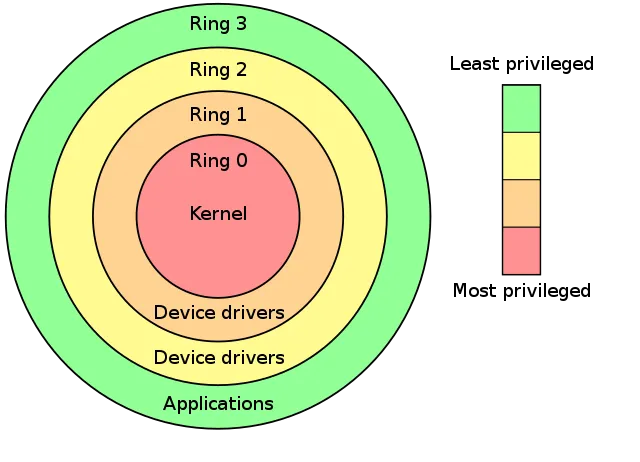
\includegraphics[width=\linewidth]{rings.jpg}
  \caption{\small Distribucion jerarquica de los  privilegios.}
  \label{fig:etiqueta}
\end{figure}
\newline
Cada modo tiene una región de memoria mapeada diferente; ese aislamiento está dado por la \textbf{virtualización de la memoria}\cite{Virtualizacion}. Por lo tanto, el modo usuario no puede acceder a la misma información que el modo kernel, al menos de manera directa.

El \textbf{modo usuario} es el responsable del anillo 3, el cual solo ejecuta código a nivel software. Es decir, está aislado tanto del sistema operativo como del kernel; sus recursos son limitados y, por cada intento de modificación de memoria, manejo de archivos o contacto con el hardware, se realiza una \textbf{syscall}. Estas llamadas al sistema permiten al programa cambiar al modo kernel, dejando que el sistema operativo termine con las instrucciones necesarias y luego vuelva al modo usuario sin violar la seguridad.
De aquí podemos deducir que, en el anillo de nivel 0, se ejecuta únicamente código a nivel kernel. Este nivel es administrado por el \textbf{modo kernel} y es el nivel de seguridad más importante. El modo kernel tiene contacto directo con el hardware, es decir, tiene acceso a todo el mapeado de la memoria, incluidas las tablas de páginas, donde se encuentra nuestra información más sensible, como contraseñas, credenciales y demás datos privados.
Por lo tanto, el principal problema aquí es que, si algún programa malicioso llegara a ejecutar instrucciones en modo kernel o explotara la ejecución especulativa y fuera de orden para ejecutar instrucciones sin los privilegios necesarios, se pondría en riesgo toda nuestra seguridad, ya que podrían acceder a las páginas del kernel sin siquiera tener los privilegios adecuados.

\section{Vulnerabilidades}

La seguridad de los sistemas puede verse comprometida por distintos tipos de vulnerabilidades. En este artículo, haremos hincapié en los \textbf{ataques de canales laterales}\cite{Side Channel Attack} (del inglés Side Channel Attacks), que explotan información derivada de las condiciones físicas o lógicas durante la ejecución de un sistema para extraer datos sensibles.

¿A qué nos referimos con "condiciones físicas y lógicas"? A que estos ataques no se basan en vulnerabilidades directas en algoritmos o software, sino en la medición de:

    \textbf{Condiciones físicas}: Fenómenos observables en el hardware, como el consumo de energía, el tiempo de ejecución de operaciones o las emisiones electromagnéticas/acústicas.

    \textbf{Condiciones lógicas}: Los comportamientos de la implementación del sistema, como el estado de la memoria caché, el mapeo de memoria o los patrones de acceso a recursos compartidos.

Estas fugas de información indirecta son los llamados \textbf{canales laterales}, que permiten al atacante obtener datos secretos sin acceder directamente a ellos. \newline
%Dos de los casos mas conocidos de estos tipos de \textit{\textbf{exploits}} son \textbf{Meltdown} y \textbf{Spectre} que se detallaran a continuacion:
Existen muchismos casos de canales laterales que se pueden explotar\cite{Side Channel tipos} pero en este informe solo vamos a dentrar en el canal de temporizacion de cache (cahce timing side-channel), el cual es utilizado por Meltdown y Spectre.
                                                                  %ref[casos de canales laterales]
%ref: Introduction to Side-Channel Attacks; Paul Kocher, Joshua Jaffe, Benjamin Jun. ---- 
\subsection{Spectre}
Spectre es una vulnerabilidad que explota la ejecución especulativa para engañar al procesador y hacer que acceda a datos sensibles en la memoria, rompiendo el aislamiento entre procesos.
\newline Afecta casi todos los procesadores modernos (Intel, AMD, ARM).
\newline Fue descubierto por dos equipos de investigadores: Jann Horn (Google Project Zero) y Paul Kocher, en colaboración con Daniel Genkin (University of Pennsylvania, University of Maryland), Mike Hamburg (Rambus), Moritz Lipp (Graz University of Technology) y Yuval Yarom (University of Adelaide, Data61).
\newline Funciona de la siguiente manera:
Primero, el atacante manipula la unidad de predicción de ramas del procesador para inducir una predicción incorrecta sobre las instrucciones que se ejecutarán. De esta manera, el procesador se prepara para ejecutar instrucciones especulativamente basadas en esa suposición errónea.
A continuación, el procesador, confiando en su predicción equivocada, ejecuta especulativamente instrucciones que no debería ejecutar. Estas instrucciones pueden incluir accesos a áreas de memoria privadas, como datos de otros procesos o del sistema operativo. Aunque el procesador eventualmente detecta el error y descarta estas instrucciones, los efectos de esos accesos permanecen en la memoria caché.
Por último, el atacante explota estos efectos secundarios midiendo los tiempos de acceso a la caché con técnicas como Flush+Reload. Si el acceso a una dirección de memoria es más rápido, significa que los datos fueron cargados especulativamente y están en la caché. Si el acceso es más lento, significa que los datos no estaban en caché. A través de estos tiempos de acceso, el atacante puede reconstruir información sensible sin necesidad de acceder directamente a la memoria protegida.
\newline A continuacion, presentaremos 2 variantes de Spectre:
\subsubsection{\textbf{Spectre-PHT}}
En este tipo de ataque, el atacante manipula el predictor de saltos para que el procesador especule incorrectamente sobre una comparación en un programa.
En el siguiente codigo de C:
\begin{figure}[h]
  \centering
  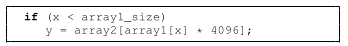
\includegraphics[width=\linewidth]{codigo_c.png}
  \caption{\small Fragmento de cdigo en C ilustrando el concepto de manipulacion de prediccion de saltos.}
  \label{fig:etiqueta}
\end{figure}
\newline x es un valor controlado por el atacante. Normalmente, el procesador verifica que x este dentro de los limites de array1, pero si el predictor de saltos ha sido entrenado para asumir que x es siempre valido, el procesador accedera a array1[x] sin verificar los limites.
Si x es un valor malicioso, puede hacer que array1[x] apunte a una direccion confidencial. Luego array2[array1[x] * 4096] almacenara esa informacion confidencial en la cache, permitiendo que el atacante lo extraiga mediante mediciones de tiempo de acceso.
\subsubsection{\textbf{Spectre-BTB}}
En esta variante, el atacante manipula la Branch Target Buffer (BTB), que es la estructura del procesador encargada de predecir el destino de saltos indirectos.
El atacante entrena el BTB para que un salto indirecto en el código del programa víctima se redirija erróneamente a una ubicación de código que el atacante elige. Esta ubicación puede contener una secuencia de instrucciones (un "gadget") que filtra información confidencial a través de la caché.
\subsection{Meltdown}
Meltdown es una vulnerabilidad que permite a un atacante acceder a la memoria protegida del sistema, incluyendo la memoria del kernel, rompiendo los mecanismos de aislamiento entre aplicaciones y el sistema operativo.
\newline Fue descubierto por tres equipos diferentes: Jann Horn (Google Project Zero), Werner Haas y Thomas Prescher (Cyberus Technology) y Daniel Gruss, Moritz Lipp, Stefan Mangard y Michael Schwarz (Graz University of Technology).
\newline Esta vulnerabilidad afecta principalmente a los procesadores Intel fabricados desde 1995, aunque ciertas variantes también pueden impactar a algunos modelos de ARM y AMD.
\newline Funciona de la siguiente manera:
\newline Primero, el atacante manipula el programa para que el procesador cargue en un registro el contenido de una dirección de memoria secreta, a la que normalmente no tendría acceso directo.
Luego, debido a la ejecución especulativa, el procesador accede anticipadamente a la memoria caché basándose en ese contenido secreto, dejando un rastro en la caché.
Finalmente, el atacante explota este rastro utilizando la técnica Flush+Reload, que le permite monitorear la caché y detectar qué datos han sido accedidos recientemente, revelando así información confidencial.
\newline A continuacion, presentaremos 3 variantes de Meltdown:
\subsubsection{\textbf{Meltdown-P}}
Este ataque afecta a los procesadores Intel y explota una vulnerabilidad en el sistema SGX, que es una tecnologia que crea espacios seguros en la memoria donde se pueden almacenar datos confidenciales..
\newline El ataque se basa en manipular la tabla de paginas, que es un mapa que le indica al procesador que direccion tiene cada pieza de informacion. Cuando un atacante cambia alguna de estas direcciones en la tabla, se provoca un fallo de protección. Este fallo debería impedir el acceso a los datos y bloquear el sistema, pero debido a la ejecución especulativa, el procesador sigue trabajando aunque haya ocurrido un error. A pesar de detectar el fallo, el procesador continúa ejecutando instrucciones usando direcciones de memoria incorrectas, lo que hace que los datos se carguen temporalmente en la caché L1. Luego el atacante puede usar la tecnica flush+reload para extraer esta informacion.
\subsubsection{\textbf{Meltdown-NM}}
Este ataque aprovecha cómo la CPU maneja de manera ineficiente los registros de la unidad de punto flotante (FPU) al cambiar de un proceso a otro. En lugar de guardar los registros de inmediato cuando se cambia de proceso, la CPU los marca como "no disponibles" y los guarda solo cuando se vuelven a utilizar.
\newline
El ataque se desarrolla en tres pasos:
\newline 1- La víctima carga datos en la FPU.
\newline 2- La CPU cambia al atacante y marca la FPU como "no disponible".
\newline 3- El atacante ejecuta una instrucción que usa la FPU, lo que genera una excepción. Sin embargo, antes de que la CPU detenga la ejecución, ya ha procesado temporalmente instrucciones usando datos de la víctima.
\newline De esta manera, el atacante puede aprovechar los datos no guardados y extraer información sensible que se encontraba en los registros de la FPU, sin tener acceso directo a ella.
\subsubsection{\textbf{Meltdown-PK}}
Los procesadores Intel Skylake-SP para servidores incluyen una función de protección de claves de memoria (PKU), que permite modificar los permisos de acceso a páginas de memoria dentro de un proceso sin necesidad de realizar una llamada al sistema o al hipervisor. Esto facilita un aislamiento eficiente de datos sensibles.
\newline Meltdown-PK es un ataque que evade las restricciones de lectura y escritura impuestas por PKU. Aunque un atacante no tenga permisos para modificar los permisos de acceso con la instrucción wrpkru, puede explotar la ejecución especulativa del procesador para acceder temporalmente a datos protegidos y filtrarlos a través de un canal encubierto.

\section{Mitigaciones}
Las vulnerabilidades de Spectre y Meltdown surgen como consecuencia directa de optimizaciones en los procesadores modernos. Aunque estas tecnicas se enfocan en mejorar el rendimiento, tambien han introducido riesgos de seguridad que han permitido el desarrollo de ataques capaces de comprometer la seguridad de los sistemas.

Dado que el problema esta relacionado con el diseño de la arquitectura de los procesadores, no tendremos una solucion definitiva hasta que el hardware sea modificado. Sin embargo, debido al tiempo que toma el desarrollo y fabricacion de nuevos chips, podrian pasar varios años antes de que las futuras generaciones de CPUs solucionen completamente el problema.

Mientras tanto, se han desarrollado diversas mitigaciones a nivel de software y hardware que pueden controlar algunas variantes de estas vulnerabilidades y minimizar el riesgo de ataques en sistemas actuales, en este informe vamos a listar algunas de las mas relevantes.

\subsection{Aislamiento de Tablas de Paginas y Aleatoridad}
El kernel se encarga de establecer tablas de páginas para controlar la asignación entre una dirección virtual y una dirección física. El acceso entre el núcleo y el espacio de usuario también se controla mediante las tablas de páginas. Una página que está mapeada para el kernel no es accesible desde el espacio de usuario, aunque el núcleo normalmente puede acceder al espacio de usuario.

Traducir los mapeos puede ser costoso, por lo que el hardware tiene un búfer de traducción de direcciones (TLB) para almacenar asignaciones. A veces es necesario eliminar las asignaciones antiguas (invalidar el TLB), pero hacerlo es costoso, por lo que el código se escribe para minimizar tales llamadas. Un truco aquí es mantener siempre las tablas de páginas del núcleo mapeadas cuando los procesos de usuario se están ejecutando. Los permisos de la tabla de páginas impiden que el espacio de usuario acceda a las asignaciones del kernel, pero el núcleo puede acceder a ellas inmediatamente cuando se realiza una llamada al sistema.

\noindent Exploits como Meltdown demostraron que este método de mantener las tablas de páginas del kernel disponibles en el espacio de usuario es vulnerable, si bien no permite directamente la filtración de información del núcleo, puede ser explotado por atacantes. Estos generan intentos de lectura sobre dichas páginas; al no contar con los permisos necesarios, la CPU bloquea el programa por seguridad (ya que se está ejecutando en modo usuario). Sin embargo, la CPU prebusca los datos de todas formas y no los desecha, por lo que quedan en la cache. Este comportamiento es aprovechado por los atacantes para medir el tiempo de acceso a los datos prebuscados y, de esta manera, llevar a cabo un ataque de canal lateral basado en caché.

\subsubsection{\textbf{Mitigacion Meltdown}}
\noindent  Para mitigar vulnerabilidades explotadas por ataques de canal lateral como Meltdown, se implementó \textbf{Kernel Page Table Isolation}\cite{PTI,Aleatorización}. Fue un cambio total en la gestión de memoria, en lugar de compartir una única tabla de páginas con el kernel, ahora cada aplicación tiene dos conjuntos de tablas de páginas -fig.4, y el sistema cambia entre ellas en cada transición entre el modo usuario y modo kernel. Cuando el código en modo usuario intenta acceder a una dirección del núcleo,no va a encontrar una direccion válida en la tabla de páginas, evitando así la explotación de Meltdown -Fig.3.
\noindent Pero este cambio tiene un gra impacto en el rendimiento. Por cada cambio de contexto (syscall, interrupciones y excepciones), se deben intercambiar las tablas de páginas, lo que implica limpiar el \textbf{buffer de traducción de direcciones} (TLB). y cuando este es  vaciado, el procesador debe recorrer las tablas de páginas en memoria para encontrar la dirección física correspondiente, lo que puede ser entre 10 y 100 veces más lento en caso de fallos de TLB. Este impacto se nota mucho en aplicaciones con llamadas al sistema frecuentes, como las que manejan big data, redes o almacenamiento intensivo.
\noindent                                                                                                                                                                                                               %ref[]
\noindent En los procesadores mas actuales, este problema se mitiga mediante \textbf{Process Context Identifiers}\cite{PCID} (PCID), esta funcionalidad asocia cada entrada del TLB con un conjunto de tablas de páginas específico. Los intercambios de tablas de páginas no eliminan completamente el TLB, por lo tanto reducen la penalización de rendimiento de KPTI sin romper la seguridad.
                                                                          %ref[]
\begin{figure}[h]
  \centering
  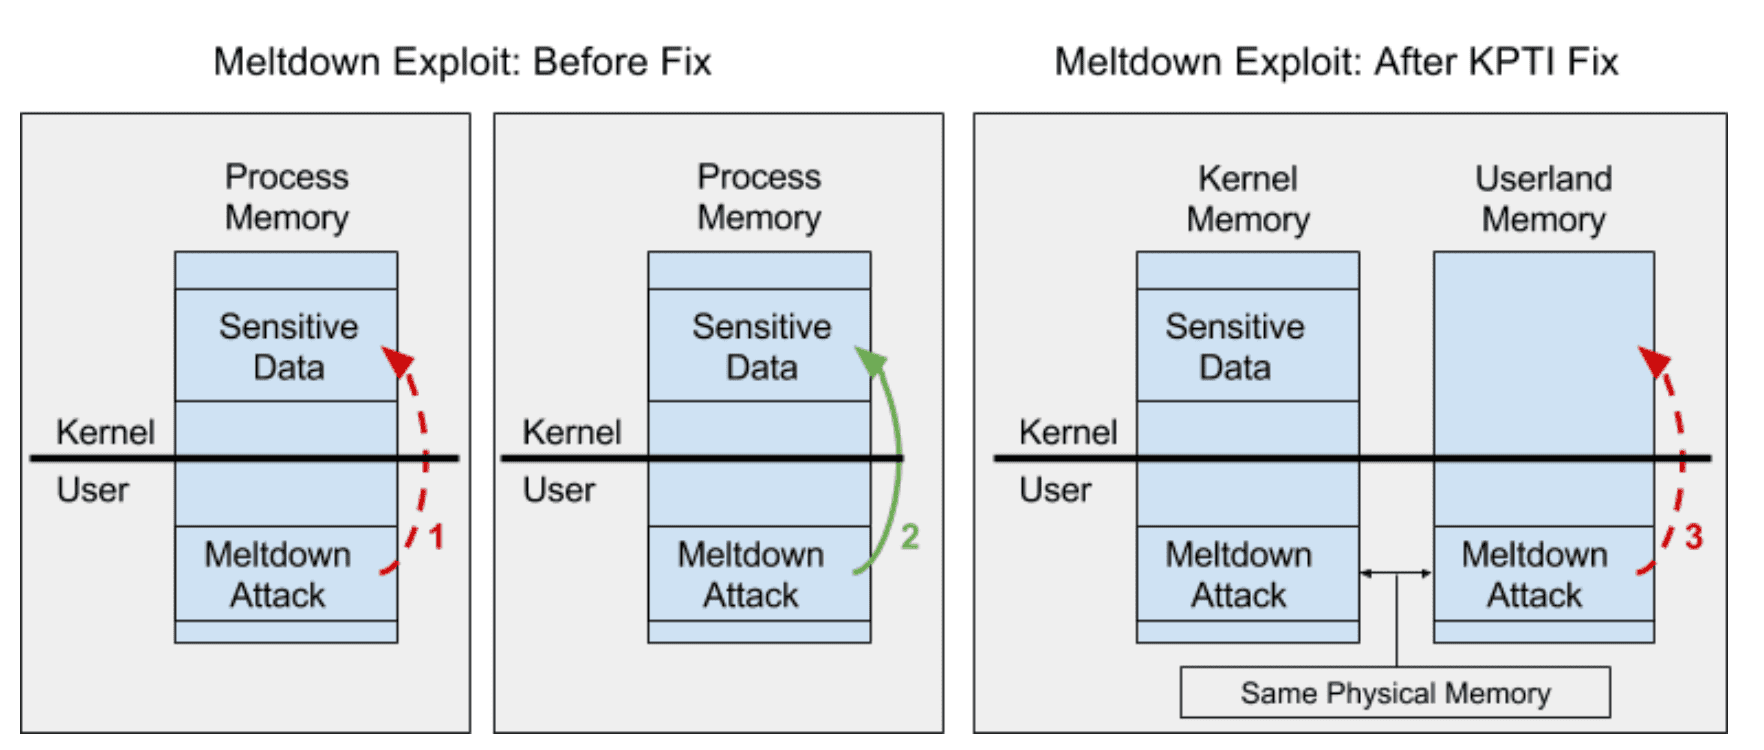
\includegraphics[width=3.5in]{kpti-meltdown.png}
  \caption{\small Ilustracion de como Meltodown intenta vulnerar las tablas de paginas antes y despues de utilizar KPTI.}
\end{figure}

\begin{figure}[h]
  \centering
  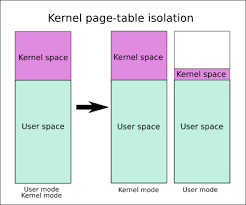
\includegraphics[width=3.5in]{isolation-page.png}
  \caption{\small Imagen representativa de como se modifican las tablas del modo usuario y kernel, luego de aplicarle el aislamiento.
  \newline
  Fijese que en las tablas del modo usuario aun quedan algunas paginas del modo kernel, esto se debe a que el sistema operativo necesita acceso a ciertas paginas del nucleo para el correcto funcionamiento del programa y utilizar mecanismos como las syscall para la interacciones entre los dos modos.}
\end{figure}

\subsubsection{\textbf{KASLR}}
\noindent Otra estrategia de defensa es \textbf{Kernel Address Space Layout Randomization}\cite{KASLR} (KASLR), se basa en aleatorizar la dirección donde se carga el kernel en memoria, haciendo mas dificil que los atacantes predigan su ubicación y hagan ataques basados en ejecución especulativa o acceso a caché.   Esta estrategia aleatoriza las direcciones en cada arranque del sistema, eligiendo dinámicamente una ubicación para el núcleo.
\noindent                                           %ref[]
\noindent Para la implementación, se han desarrollado técnicas como los parches de Cook, que modifican el proceso de arranque para determinar la dirección más baja segura en la que puede colocarse el kernel. Luego, el sistema recorre las regiones de memoria e820 y cuenta los espacios del tamaño adecuado para el kernel. A partir de estos espacios, se elige uno al azar utilizando la mejor fuente de números aleatorios disponible, ya sea la instrucción RDRAND, los bits menos significativos del contador de tiempo RDTSC o bits de los puertos de E/S del temporizador. Una vez seleccionado el espacio, el kernel se descomprime, se maneja la reubicación y se inicia el sistema.
\noindent
\noindent De esta manera, no solo se aísla el acceso a las páginas del kernel con KPTI y KASLR sino que tambien se asegura que la ubicación del kernel en memoria sea impredecible en cada arranque. 

\noindent Sin embargo, aunque estas técnicas reducen significativamente la efectividad de ataques como Meltdown y Spectre, no son soluciones definitivas. Ataques de canal lateral más sofisticados pueden seguir filtrando información del kernel a pesar de estas mitigaciones, lo que ha llevado a la investigación de nuevas estrategias de defensa, tanto en software como en hardware.
                                                                                                                                                                                                                                                                                                                                                                                                                                 %ref[bitbreaks]                             

\subsection{Retpoline}
El nombre Retpoline es un acrónimo de “return” (retorno) y “trampoline” (trampolín). En este contexto, un trampolin es un pequeño fragmento de codigo invocado como funcion, que realiza una tarea breve y, a diferencia de una llamada a funcion comun, no regresa a su llamador despues de la ejecución, sino que salta a otra ubicacion, como se muestra en la Figura 3. Si el destino del salto del trampolin es una funcion, al retornar, dicha funcion regresara al llamador original del trampolin.
\begin{figure}[h]
  \centering
  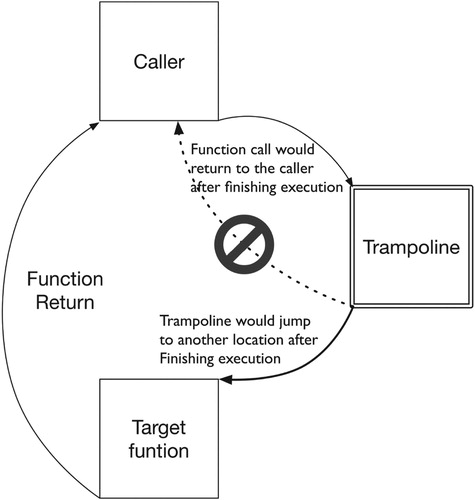
\includegraphics[width=\linewidth]{retpoline.jpg}
  \caption{\small Trampoline se refiere a un fragmento de código que saltaría a otra ubicación después de terminar la ejecución en lugar de regresar al llamador original.}
\end{figure}

Retpoline fue desarrollado por Google para mitigar los ataques Spectre-BTB. Su objetivo es evitar que este tipo de ataques manipulen el Branch Target Buffer (BTB) y desvien la ejecucion especulativa hacia una direccion arbitraria. Para ello, Retpoline reemplaza las bifurcaciones indirectas con una secuencia especial de instrucciones basada en llamadas y retornos, asegurando que la ejecucion especulativa permanezca en un bucle inofensivo dentro del Return Stack Buffer (RSB). Esto impide que un atacante manipule las predicciones de bifurcaciones para ejecutar codigo malicioso.

Para lograr esto, Retpoline aprovecha la forma en que los procesadores gestionan las llamadas y retornos de funciones. Al utilizar una instruccion call hacia un trampolin, se llena el RSB con una direccion de retorno controlada. Cuando el procesador especula sobre el retorno, en lugar de seguir una prediccion potencialmente manipulada desde el BTB, sigue la direccion almacenada en el RSB y ejecuta un bucle de instrucciones seguras.
%https://www.tandfonline.com/doi/epdf/10.1080/02564602.2018.1531072?needAccess=true

\begin{thebibliography}{9}


\bibitem{paralelismo} Paralelismo en las instrucciones, [Disponible]: \url{https://orgacomp.github.io/9557/teoria/procesador/paralelismo/}

\bibitem{Virtualizacion} Cap 9, Computer Systems: A Programmer’s Perspective (3.ª ed.) 2015 , Pearson.
\bibitem{syscall}  Linux system calls,” 2019. [Disponible]: \url{http://man7.org/linux/man-pages/man2/syscalls.2.html} 
\bibitem{Aleatorización} Aleatorización del diseño del espacio de direcciones del núcleo, [Disponible]: \url{https://bit.ly/aleatorizacion-kaslr}
\bibitem{PTI} Page Table Isolation, The Linux Kernel, [Disponible]: \url{https://bit.ly/PageTableIso}.
\bibitem{Rendimiento-Parches} Performance Impact of Host Kernel Page Table Isolation on Virtualized Servers, 2021, Song Wei; Kun Zhang; Bibo Tu, [Disponible]: \url{https://ieeexplore.ieee.org/document/9421326}
\bibitem{Side Channel Attack} Introduction to Side-Channel Attacks; Paul Kocher, Joshua Jaffe, Benjamin Jun.
\bibitem{Side Channel tipos} Power Analysis Attacks: Revealing the Secrets of Smart Cards, 2007,  Stefan Mangard, Elisabeth Oswald, Thomas Popp.
\bibitem{KASLR} KASLR in the age of MicroVMs, 2022, [Disponible]: \url{https://www.cc0x1f.net/publications/kaslr.pdf}
\bibitem{PCID} Process Context IDentifiers, [Disponible]: \url{https://www.kernel.org/doc/Documentation/x86/pti.txt}, \url{https://bit.ly/pciddoc}
\bibitem{meltdown} Lipp, M., Schwarz, M., Gruss, D., Prescher, T., Haas, W., Fogh, A., Horn, J., Mangard, S., Kocher, P., Genkin, D., Yarom, Y. y Hamburg, M. (2018). Meltdown: Reading Kernel Memory from User Space. In *27th USENIX Security Symposium (USENIX Security 18)*.

%\bibitem{Exploits-Parches} Linux kernel exploit development, 2022. [Disponible]: \url{https://breaking-bits.gitbook.io/breaking-bits/exploit-development/linux-kernel-exploit-development}
%\bibitem{TLB} Memory system, 2016, Sarah L. Harris, David Money Harris, in Digital Design and Computer Architecture, 2016. [Papers]:\url{https://www.sciencedirect.com/topics/computer-science/translation-lookaside-buffer}


\end{thebibliography}


\end{document}

